\documentclass[12pt, a4paper]{article}

\usepackage[T1]{fontenc}
\usepackage[utf8]{inputenc}
\usepackage{libertinust1math}

\usepackage{csquotes}
\usepackage[english]{babel}
\usepackage[backend=biber, style=apa, sorting=nyt]{biblatex}
\addbibresource{final.bib}

\usepackage{graphicx}
\usepackage{subcaption}
\graphicspath{{./assets/}}

\title{The distribution of Rust contributors: An analysis of a relatively young language}
\author{Joshua Megnauth}
\date{\today}

\begin{document}
\maketitle

\section{Introduction}
Open source software is a unique phenomenon in terms of multiple areas of study including philosophy, sociology, political science, software development, and others. Mass, open cooperation is an immensely difficult proposition. Yet "the world runs on open source" is a common refrain that refers to the uncontroversial notion that free software is everywhere (\cite{fossdatasci2020}). Linux and FreeBSD run most of our software which in turn run open source servers. Middleware libraries such as OpenSSL glue together systems. Even consoles, such as every PlayStation beyond PlayStation 2, run on open source kernels. Sony notably uses FreeBSD in their consoles (\cite{ps4freebsd}).

Free software's openness and prevalence alone makes research enticing. However, another factor is version control systems, like \textit{Git}, coupled with public sites that host projects such as \textit{GitHub} or \textit{GitLab}. GitHub and others host or mirror thousands of projects with a range of sizes. Much of the data on users, projects, and the projects they contribute to are public. The data are rich consisting of dates and times, textual data on conversations about contributions, as well as the heavily layered contributions themselves.

One of the most interesting projects on GitHub is the Rust programming language. Rust is developed in a transparent manner with Requests For Comments (RFCs) posted on GitHub (\cite{rustrfcs}). The majority\footnote{At least since 2011. Older Rust development from back when the language was a side project may be available somewhere.} of Rust's development from its early days to everything from Rust's current state is visible on GitHub (\cite{rustmainrepo}). The merits of new language features or changes are discussed fairly publicly with recorded meetings available on issues (\cite{rustteammeets}). Finally, Rust is a relatively new programming language that takes aim at a stalwart, C as well as C++, C's classy sibling. That fact is not important by default, but Rust actually has momentum while challenging C which is perhaps one of the most fascinating recent developments in software development. For example, developers on Stack Overflow, a platform used to ask programming questions, voted Rust as their favorite language for four years in a row (\cite{stackoverflowdevsurvey2020}). Mozilla has successfully ported some of Firefox's code from C++ to Rust---a process colloquially called \textit{oxidation}.

All of this is to say that the enterprising computational social scientist is able to more or less track Rust's development over at least a decade. Said scientist is able to watch contributors work on an exciting, growing language as well as work on important libraries used in the ecosystem, such as Serde. Researchers may focus on different areas depending on their interests. Open source has elements of anarchism, democracy, socialism, as well as liberalism depending on whom one asks. Thus, researchers in the humanities or the digital humanities, for example, have access to a large scale participatory program during growth. My research's route is different: complex networks. Version control systems such as Git or Subversion are perfect for network analysis since they're effectively laid out as graphs. Contributor networks function like co-posting networks as one would craft for researchers, actors, or writers.

\subsection{Research question and caveats}
Are Rust developers assortative based on whether they work on the core, middleware libraries, or projects? A relatively young language like Rust may have many people who contribute to both the core of the language as well as high profile projects. This is not the case with mature languages. The developers of well trafficked Python data science libraries such as Pandas or matplotlib don't necessarily contribute to the Python language itself. For Rust, however, I've noticed that some high profile Rust programmers also contribute back to the language. Jeremy Soller is the principal engineer of System76, a Linux laptop company. Soller is also well known within the Rust community for starting and greatly contributing to an experimental, Unix-like operating system written completely in Rust known as RedoxOS. Soller contributed back to the Rust language to fix issues\footnote{https://github.com/rust-lang/rust/search?q=jackpot51\&type=commits} encountered when working on Redox (\cite{lunduke31317}). Another excellent example is BurntSushi (Andrew Gallant). BurntSushi is involved in the core development of the language but is also known for developing the world's fastest \textit{grep}---\textit{ripgrep}, programmed in Rust---which Microsoft uses in Visual Studio Code (\cite{gallant2016}).

I faced some notable limitations with my research which I'll discuss in a limitations section. Currently, I consider my research to be something of a toy project that should be repeated with more data. However, my open source code should be sufficient to repeat and extend the project.

As a nascent but growing language, studying the graph of Rust contributors is thus novel as well useful for the social sciences. Open source projects can be rather dramatic at times leading to controversial forks. Forks such as pfSense/OpnSense, OpenSSL/LibreSSL, FFmpeg/libav, Nexuiz/Xonotic, OpenOffice/LibreOffice, and many others were the result of disagreements rather than good spirited splits. However, Rust is a stable project where additions and new ideas seem to encounter less friction than some other projects. Future studies could focus on the elements that seem to help Rust avoid controversies and bad blood.

\section{Background: Rust and GitHub analysis}
\subsection{Rust}
Rust is a systems programming language that draws inspiration from OCaml, Haskell, C++, Erlang, Ruby, and others (\cite{rustlang}). Rust's guiding principal is memory safety based on fixing the unsafe qualities of languages like C. C is sometimes described as a "cowboy" language or a language full of "foot-guns." C is full of undefined behavior that the language trusts the programmer to avoid. The language is similarly reticent to complain about incorrect memory access, such as going beyond the bounds of a buffer. C offers extreme power but exacts a mental toll on programmers that must be hyper aware of the implications of their code. Even the best programmers continue to write code that is memory unsafe due to the extreme difficulty of getting it right. Use after free, buffer overflows, dereferencing null pointers, non-thread safe variables, double free, et cetera are all still common and happen by accident more than ignorance (\cite{hosfeltsafety2019}). The Chromium project notes that 70\% of their bugs are related to memory issues that Rust would solve (\cite{chromiummem70}). Rust piqued Mozilla's interest for the same reason which is why they adopted the language with gusto. Mozilla, as mentioned earlier, has rewritten sections of Firefox in Rust over time to catch unsafe behavior at compile time (\cite{hosfeltrewrite2019}). Other companies, including Microsoft (\cite{microsoftrust2020}), Apple (\cite{applerust2020}), and Amazon (\cite{amazonrust2020}), are also writing core infrastructure in Rust.

Rust is notoriously difficult due to a mechanism known as the \textit{borrow checker}. The borrow checker is something of a static analysis tool that imposes restrictions on the access and mutability of data. Essentially, unlimited immutable borrows are allowed. Only one mutable borrow is allowed. An immense amount of potential errors are caught with these two rules. Rust types are also labeled whether they may be safely sent across threads---and the borrow checker applies to threading as well. Programmers are often surprised at how often they write unsafe memory accesses. With all of that said, Rust aims to be as fast or faster than C. Rust is built on explicitness and zero cost abstractions. Like C and C++, programmers don't pay for what they don't use. The language forms a strict separation between safe and unsafe code which makes unsafe code\footnote{Unsafe code is unavoidable in some contexts.} easier to debug. Rust's strong functional background means that the language precludes classes; Rust is only OOP if you squint and add qualifiers to your definition. Programming in Rust feels far more ergonomic when an idiomatic style of composition and lambda calculus is used rather than trying to build up a C++ or Java style class system. Thus, many nascent Rustaceans\footnote{Rustacean is the demonym for Rust programmers.} are initially turned off when they attempt to write Rust code like one would for C. Seemingly innocuous lines of code fail to compile because, say, a variable is not handled in a thread safe manner despite being used in a multithreading context. Another example is the case of floating points. Floating point values are infamously tricky to work with so Rust places restrictions on certain equality statements for floats (\cite{programmingrust}).

\subsection{GitHub analysis}
GitHub is a platform that hosts open source projects. The "Git" in GitHub refers to Git, a version control system developed by Linus Torvalds for Linux. Version control systems track file changes to make pushing and pulling changes quicker. Git is designed to ease the process of multiple programmers\footnote{Though Git isn't limited to code!} working on the same project at once. GitHub leverages Git but with a slick web interface and social features. Prior to GitHub, a somewhat clunky site hosted a wide array of commonly used open source software. GitHub's original goal was decentralization---other services arose around the same time as well. However, GitHub won out by virtue of modernity rather than simply being a stable host of open source projects (\cite{metz2015}).

GitHub research fall concretely into the computational social science camp. Data are usually scraped due to the presence of an API and the ease of retrieving the required data rather than depending on finding a large precompiled data set. Researchers deploy techniques such as natural language processing, graph theory, or machine learning.

Yue Yu, Huaimin Wang, Gang Yin, and Tao Wang studied the effect of pull requests on development. Contributors work on a feature or bug fix locally then send a request to a project's team to pull the contributor's changes upstream. Yu et alia explain that the barrier to contributions are relatively low due to the PR system. Any user may potentially contribute bug fixes, features, documentation updates, et cetera. However, assigning bug fixes to contributors or choosing a reviewer for a PR is labor intensive. The researchers specifically focus on GitHub rather than other services with git as its core. The researchers tested several methods of assigning PRs to reviewers using a GitHub comment network based on pull requests. For example, PRs were assigned in their model based on contributor and reviewer similarities. Another tested method compared the similarities of file paths to determine a reviewer based on the issues they usually handle. The researchers found that their NLP comment network model performed as well as manual selection for assigning PRs. However, a mixed model approach performed the best overall (\cite{YU2016204}).

GitHub is not the first repertoire of wildly available open source software. The GNU project, Sourceforge, and the Linux mirrors all host open source software repositories. The GNU project and Sourceforge both contain a set of software rather than one project. GitHub's social features presumably induce collaboration more than Sourceforge which lacks similar mechanisms. Dorota Celi\'{n}ska researched how open source projects on GitHub gained collaborators. Ostensibly, a social network focussed on coding would facilitate recruiting new programmers and helpers. However, as GitHub hosts hundreds of millions of repositories, understanding how developers connect is pivotal. Celi\'{n}ska's three hypotheses were that reputation, reciprocity, or programming language popularity would affect gaining collaborators. Reputation (especially followers count) and reciprocity increased the probability of collaboration (\cite{celinska2018}).

Collaboration is great, but end users expect good software not just collaboration. Oskar Jarczyk et alia updated research on the quality of developed projects. The two main metrics were commits (submissions) as well as bug fixes. Interestingly, the researchers found that different forces contribute to each metric. Closing issues requires a strong core team or centralized work. However, centralized work doesn't increase commits as a whole. On the other hand, social network features and network metrics (such as skill similarity of contributors or density) positively affect the number of commits while having a mild negative effect on bug closures (\cite{JARCZYK201832}).

\section{Methodology}
\subsection{Scraping GitHub data}
\begin{figure}[ht!]
    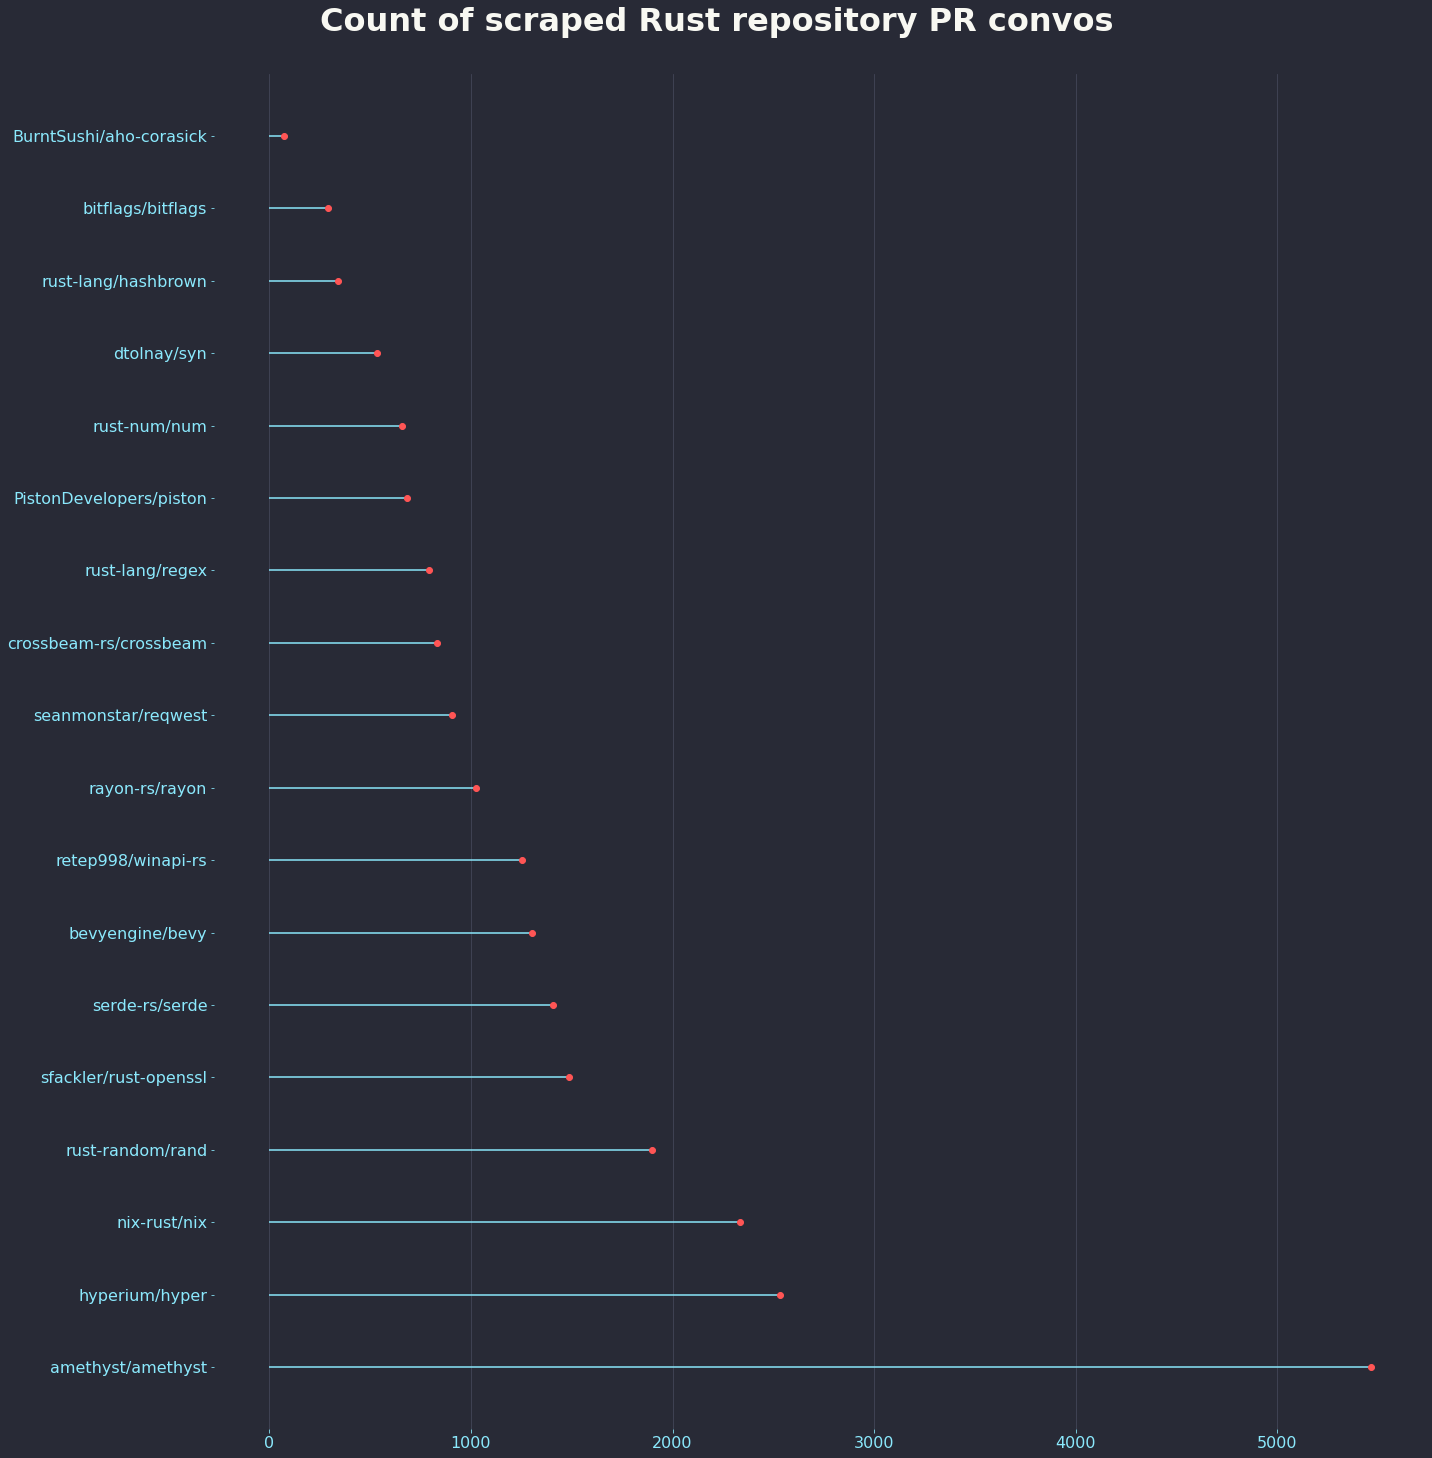
\includegraphics[width=\linewidth]{lollypopcounts.png}
    \caption{The data set contains all of the pull request conversations up to October 23 2020. The total counts are shown above.}
    \label{fig:lollycounts}
\end{figure}

The first step in analyzing GitHub data is to, of course, retrieve GitHub data. GitHub provides two public APIs, a deprecated REST API as well as a newer GraphQL API. GraphQL is a new, open source query language developed by Facebook designed to replace REST with a strongly typed, faster, and standardized system. GraphQL requests are sent and received as JSON. The actual queries are written in GraphQL (i.e. the query language) (\cite{graphql}). To gather my data, I wrote a scraper in Rust to gather the data I need and deserialize the observations to a CSV. My scraper is open source---like everything else used in this project\footnote{https://github.com/joshuamegnauth54/git-github-graphs Nota bene: My Rust is quite awful, as is most of my code.} My scraper as well as the GraphQL query are available in the footnote. The query shows \textit{exactly} which data were gathered.

With that we've reached the first potential caveat of my research. GitHub's REST API allows directly scraping the list of contributors per repository as I originally intended. However, the GraphQL port isn't yet feature complete. One of the missing features is an endpoint for scraping contributors directly. Thus, I opted to gather participants on every pull request (PR) conversation held in the repository. I essentially gathered data on anyone who contributed or attempted to contribute by submitting code or starting a discussion. This method may be superior to the traditional method of only gathering collaborators because the data contain a weight element by the number of times a person posted in a conversation. However, particularly wordy conversations would likely skew the data hence the caveat. Examining degree centrality, as discussed later, seems to disprove the skew theory because some of the users I expected to have high centrality were present. Regardless, the potential remains especially considering very chatty projects.

\begin{figure}[ht!]
    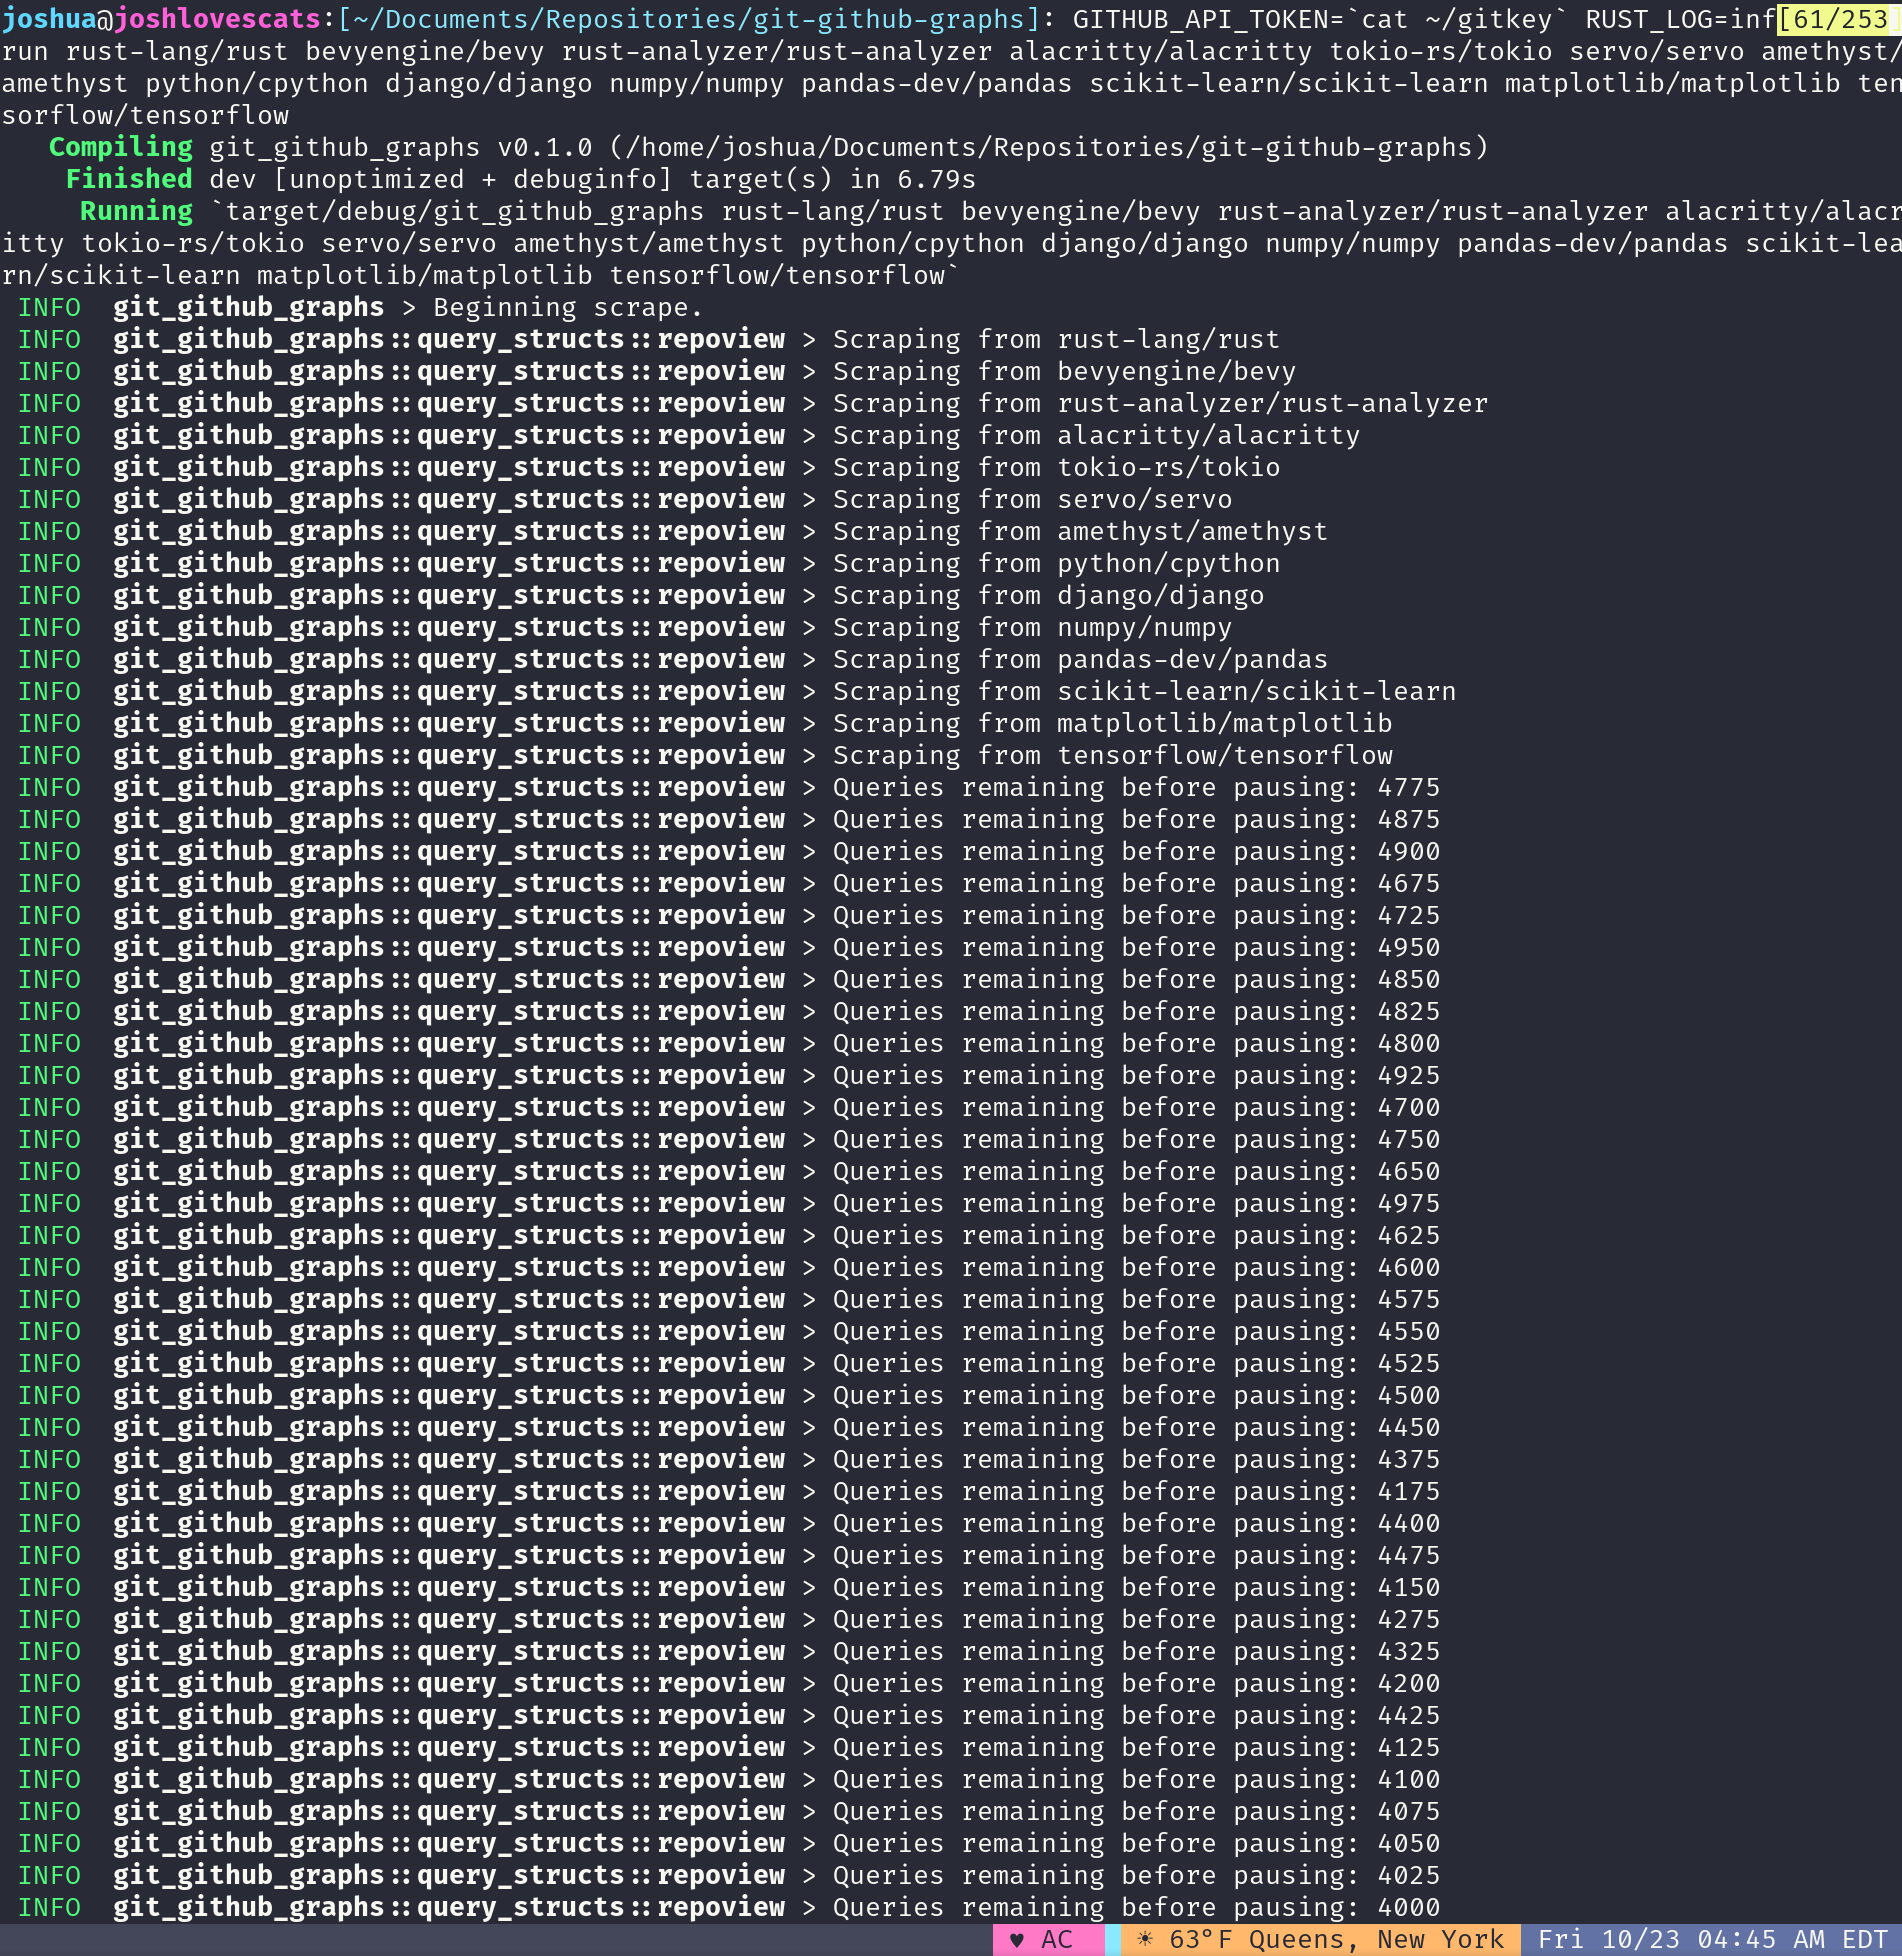
\includegraphics[width=\linewidth]{scraper.jpg}
    \caption{My scraper gathering the data used for this very paper.}
    \label{fig:scraper}
\end{figure}

The second caveat is why I proclaim my project is a toy. A list of the repositories I gathered may be found in table \ref{tab:repoinfo}. I built the list of repositories using GitHub as well as the Rust Package Repository, crates.io.\footnote{https://crates.io/}. Libraries and programs are known as "crates" in Rust parlance. I worked through the list of top projects sorted by stars on GitHub or most downloaded on crates.io. Most projects consisted of too many data points to comfortably analyze. In other words, scraping the entire project would add far too many nodes and edges to handle on a home computer even if my hardware is powerful. Server caliber hardware or distributed computing are usually recommended for big data. As a result I did not choose repositories based on a rigorously scientific method. The list consists of prevalent repositories that are manageable for analysis---a value judgement based on the amount of PRs. The list is reasonably diverse but most certainly flawed and far too small.\footnote{Ironically, I scraped 127000 observations for my thesis which my computer handled fine. I found gauging how much data to scrape difficult and thus scraped far too little data here. However, all of the criticisms would hold with more data as well.}

\begin{table}
    \centering
    \begin{tabular}{ccc}
        \hline\\
        Repository & Description & Attribute class\\
        \hline\\
        amethyst/amethyst & Data driven game engine & Project\\
        hyperium/hyper & Lower level HTTP library & Library\\
        nix-rust/nix & Unix API bindings & Core\\
        rust-random/rand & Pseudorandom numbers library & Library\\
        sfackler/rust-openssl & Rust OpenSSL bindings & Core\\
        serde-rs/serde & Serialization and deserialization library & Library\\
        bevyengine/bevy & Newer (2020) ECS game engine & Project\\
        retep998/winapi-rs & Windows API bindings & Core\\
        rayon-rs/rayon & Data parallelism toolkit & Library\\
        seanmonstar/reqwest & High level HTTP client; uses hyper & Project\\
        crossbeam-rs/crossbeam & Tools for concurrent programming & Library\\
        rust-lang/regex & Regular expressions & Core\\
        PistonDevelopers/piston & Modular game engine & Project\\
        rust-num/num & Higher precision numbers & Library\\
        dtolnay/syn & Parses a stream of Rust syntax & Core\\
        rust-lang/hashbrown & Google's SwissTable algorithm in Rust & Core\\
        bitflags/bitflags & Generates structs that manage bit flags & Library\\
        BurntSushi/aho-corasick & String searching algorithm & Core\\
        \hline
    \end{tabular}
    \caption{Data were gathered from the following repositories. All pull request conversations were gathered up to October 23 2020.}
    \label{tab:repoinfo}
\end{table}

Additional metadata were gathered beyond pull request conversations and titles. The data also include:
\begin{enumerate}
    \item The date of each post
    \item Location of each poster
    \item List of organizations
    \item Poster's company
\end{enumerate}
None of these extra data points were used in the final project. Date is a useful observation. Location and company are both flawed since nodes have completely leeway over what they may enter into those fields. Thus, location, for example, is either extremely difficult to parse due to the many ways a person may enter in the same location ("New York", "New York, New York", "Queens, New York", "NY", "In my house, NY"). Location is often blank or may be set as a joke ("~/" is common). Company exhibits similar problems, but most often the field is blank. Organizations is more mandated but, again, is often blank.

\subsection{Assortativity}
Table \ref{tab:repoinfo} also lists each repository's attribute class. Calculating assortativity (homophily) requires an attribute for comparison. For example, a research may calculate assortativity based on sex, political party, et cetera. I manually assigned each repository to either Core, Library, or Project. The distinction is based on my own justifications. Two caveats are apparent here. The first is that the attributes were entirely based on my own thoughts. The second is that the data is lacking so many of the repositories may be assigned different classes if more data were gathered. More data would engender fuller, more robust categories. Additionally, more data would allow reasonably adding more classes as a whole. For example, as a low level language Rust is reasonably popular for game engines and games. Classifications for games, game engines, and graphics and sound APIs could be added if a larger graph were gathered. Other classifications, such as crates used for the internet in some way, can be added to split up the libraries class. The current libraries class does not distinguish between lower level libraries that provide, say, high precision numbers or linear algebra routines and higher level libraries. More classes would be more robust due to granularity.

Core, library, and project are coarsely defined classes. I define core as projects are either directly part of Rust or unofficially a central project. Regex is not an official part of the Rust standard library, but the regex crate is developed by the Rust Project Team and exists under the "rust-lang" account. Thus, I labelled regex as core. Crossbeam is a library of tools for concurrent programming such as thread safe queues, message passing interfaces, atomic types, et cetera. Crossbeam is positioned as a library rather than a core project since the project isn't directly connected to the Rust language. However, libraries like Crossbeam are a big ambiguous since they seem lower level than other libraries despite not being a core project. The project class is probably the easiest to parse. Projects are relatively high level crates that use lower level libraries to produce something designed more for consumers. Ideally projects would be split into programs directly designed for end users and very high level libraries designed to make lower level libraries easier to use by encapsulating common functionality. For example, my scraper is a project\footnote{Obviously not included in the data.} that uses the reqwest and graphql-client libraries. Clearly all three of these are of different scales.

The next step is to actually process each node to add the attributes. I generated the attributes by two methodologies I call \textbf{most active repository} and \textbf{max repository}. \textbf{Max repository} is the repository the user contributed to the most personally in terms of the data. \textbf{Most active repository} is the repository among the set contributed to by the user that is most active total. As an example, consider a programmer who contributed to repositories \textit{awesome-game-engine}, \textit{amazing-cat-data}, \textit{smol-mpd-gui}, and \textit{Firefox}. The user contributed once to Firefox but 25 times to \textit{amazing-game-engine}. She contributed a handful of times to the other two repos. That programmer's \textbf{most active repository} would be Firefox simply because that's obviously the most active project. However, her \textbf{max repository} would be \textit{awesome-game-engine} because she personally contributed to that repo the most.

\subsection{Projection}
My network data have a bipartite structure. Bipartite structures exist when nodes may be split into two sets where edges exist between the two sets but not within. A simple example is a product network. Customers buy products which leads to two disjoint node sets, Customers and Products. My network data contain \textit{authors} and \textit{pull requests}. The two sets don't overlap, but we're more interested in the connections between authors than pull requests. A graph projection allows mapping pull requests onto authors so that each author shares an edge if they commented on the same PR. The projection is weighted to account for multiple connections.

\subsection{Python code}
My code is fully open source and available on GitHub across two repositories. My thesis repository\footnote{https://github.com/joshuamegnauth54/GamerDistributionThesis2020} contains convenience functions and tools for plotting networks and calculating statistics using NetworkX. My functions are designed to encapsulate certain common tasks such as plotting with a consistent style or calculating random graph replicates. The code is written completely in Python using the NetworkX (\cite{networkx}), matplotlib (\cite{Hunter:2007}), and pandas (\cite{reback2020pandas}) libraries. Some of the code is wonky because I originally began coding for a different project. Some of the function parameters are "gamers" in some way which refers to the original network used when writing the code. However, the code is general enough to work with my Rust repositories graph as well. The repository\footnote{https://github.com/joshuamegnauth54/Data790\_PyVis/tree/main/src} for this paper, in the spirit of open and transparent science, contains the code used to load and process the network as well as how the convenience functions were called to produce the results below.

\begin{figure}[ht!]
    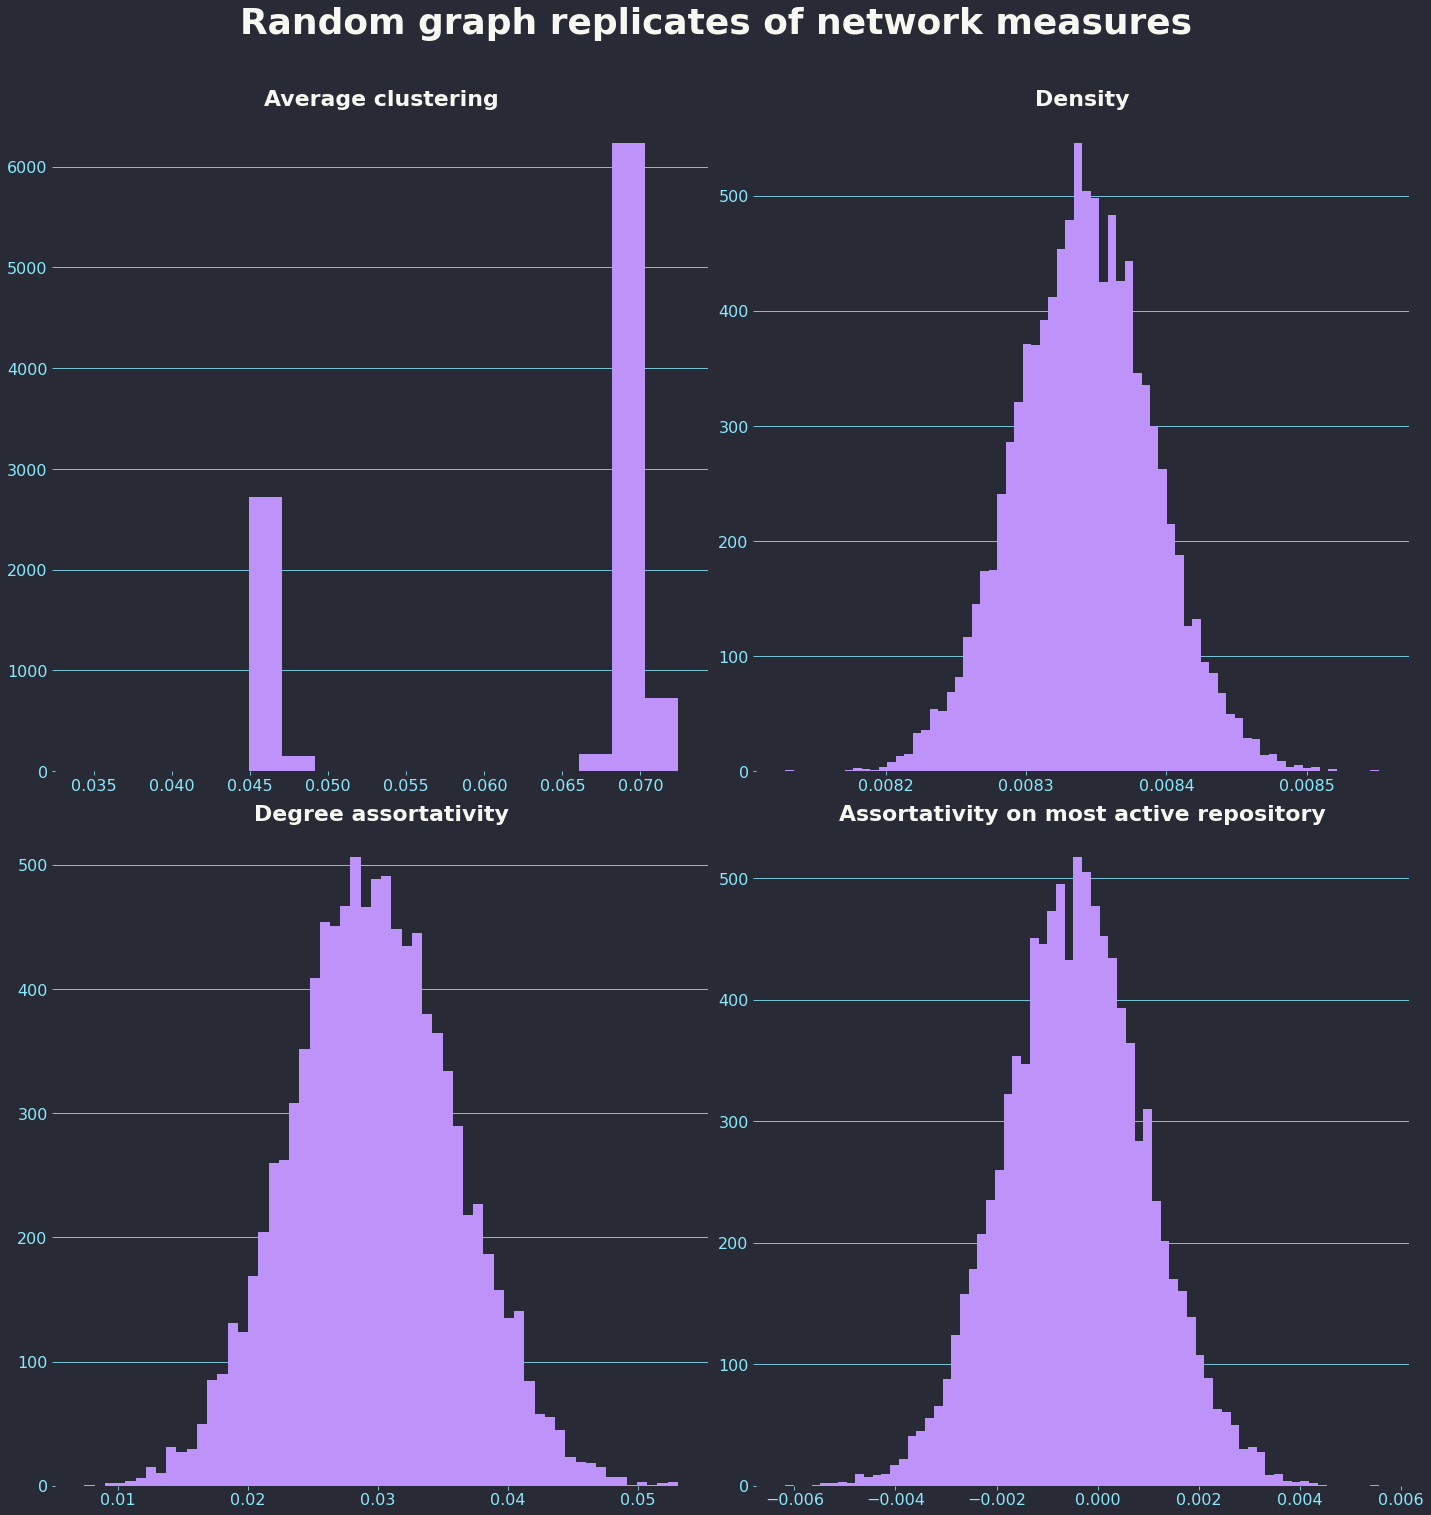
\includegraphics[width=\linewidth]{metrics_dist.png}
    \caption{Distribution of randomly calculated graph replicates without the observed statistic.}
    \label{fig:metricsdist}
\end{figure}

I calculated random graph replicates in order to compare my observed statistics to a simulated null distribution. P values are the probability of obtaining a statistic at least as extreme as what was observed. P-values are deeply flawed and don't indicate proof of anything. However, they're useful for a big picture view of the quirkiness of a statistic. The replicates were calculated by first simulating 10000 random graphs with parameters similar to my \textit{unprojected} graph. Next, I projected the simulated graph followed by calculating the requisite statistic. After 10000 repetitions of this process we end up with a distribution of random expected statistics with a visualize indication of the weirdness of our observed stat. The p-values are effectively zero at 10000 replicates but may be slightly less strange at a higher N.

\begin{figure}[ht!]
    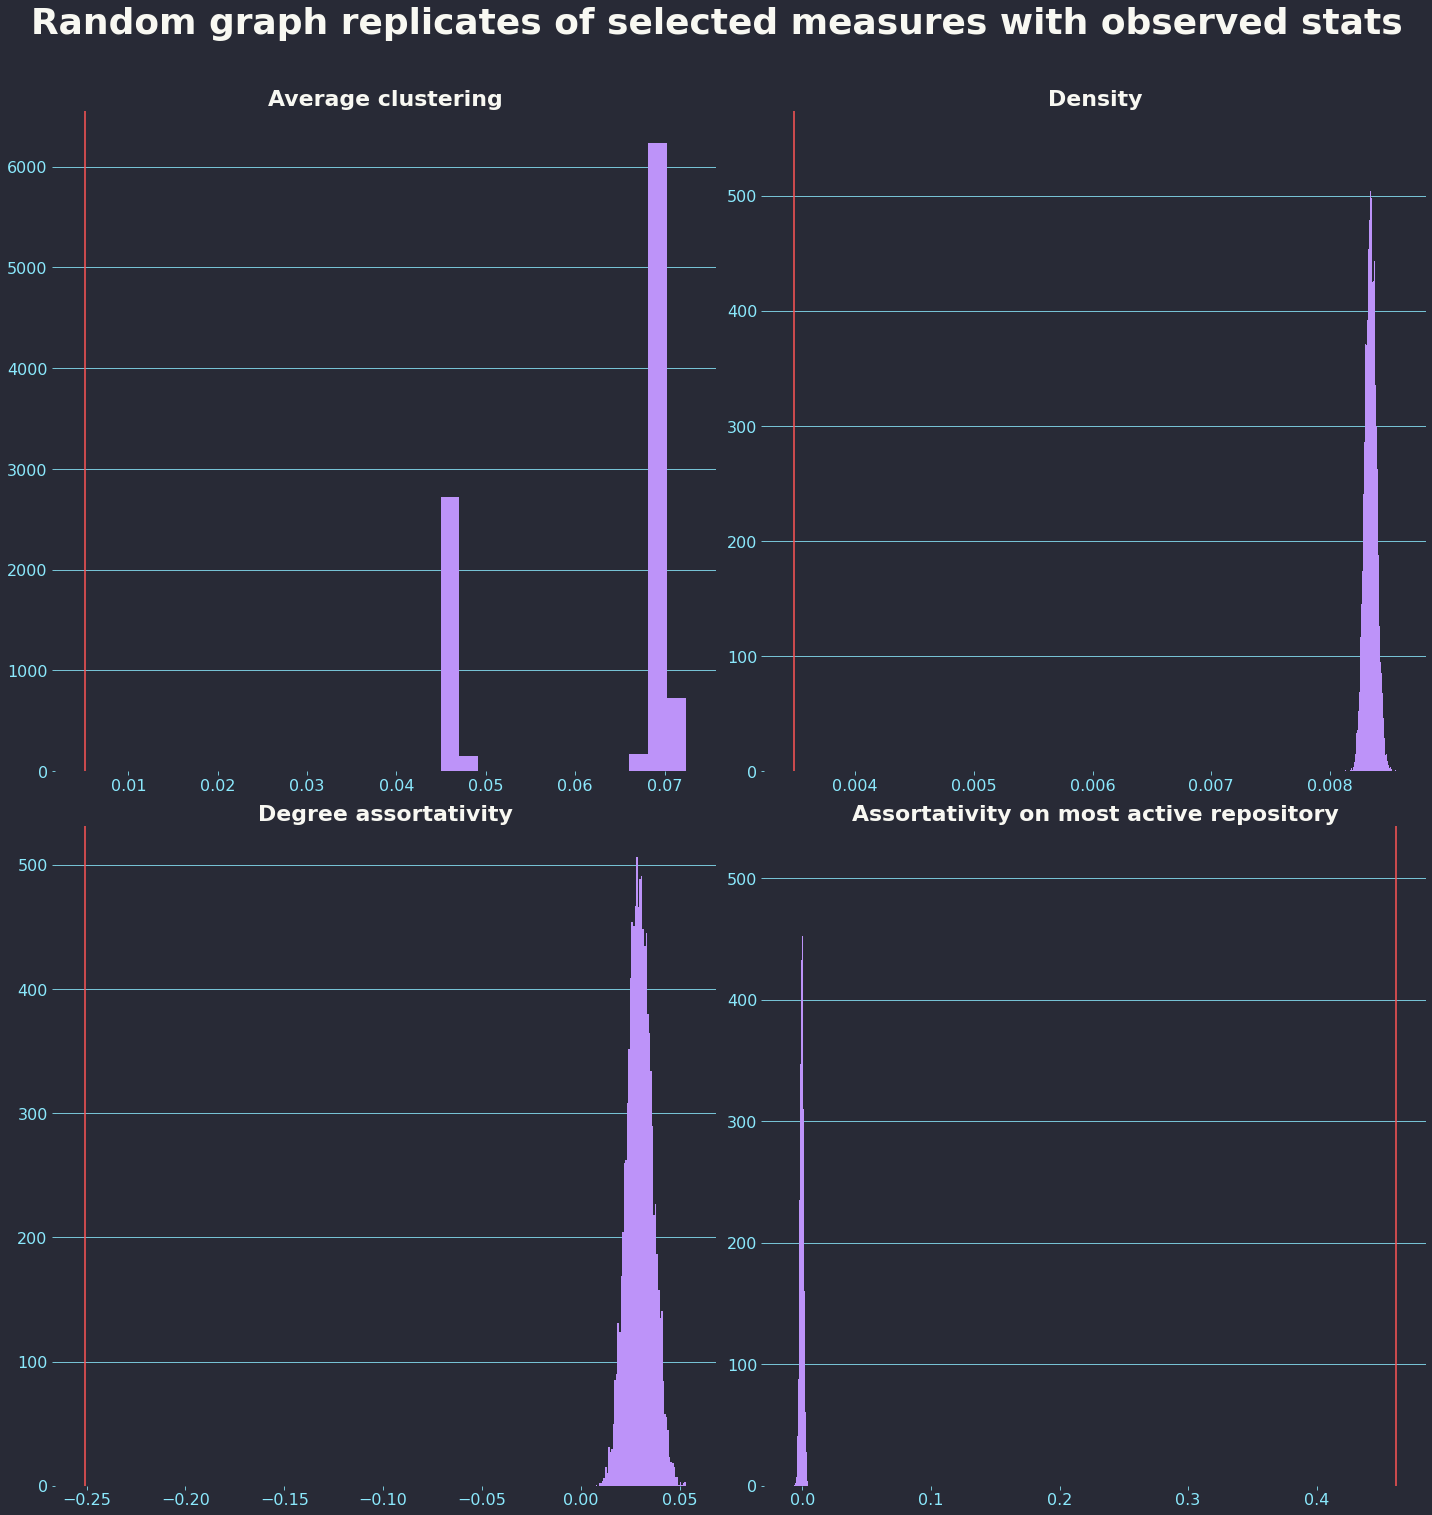
\includegraphics[width=\linewidth]{metrics_dist_w_obs.png}
    \caption{Random graph replicates with the observed statistic in red. The p-values are effectively zero at 10000 replicates.}
    \label{fig:metricswobs}
\end{figure}

\section{Results}
The first results landmark of note is the size of my full network as opposed to the largest connected component. The network is largely fully connected as only 33 nodes and one edge are present in the full network while absent from the LCC as shown in table \ref{tab:netresults}. Fundamentally, this means that the full PR network (since every node was gathered for those repos) is almost fully connected. Most nodes are reachable in some way. For a PR network this means a contributor that is connected to other contributors posted in most PR conversations. A metric like this is somewhat tautological for a PR network. Likely most PRs would have a contributor connected to other contributors responding in some way even if the PR is eventually discarded. Regardless, demonstrating mathematical proof of an "obvious" phenomenon is always useful.

\begin{figure}[ht!]
    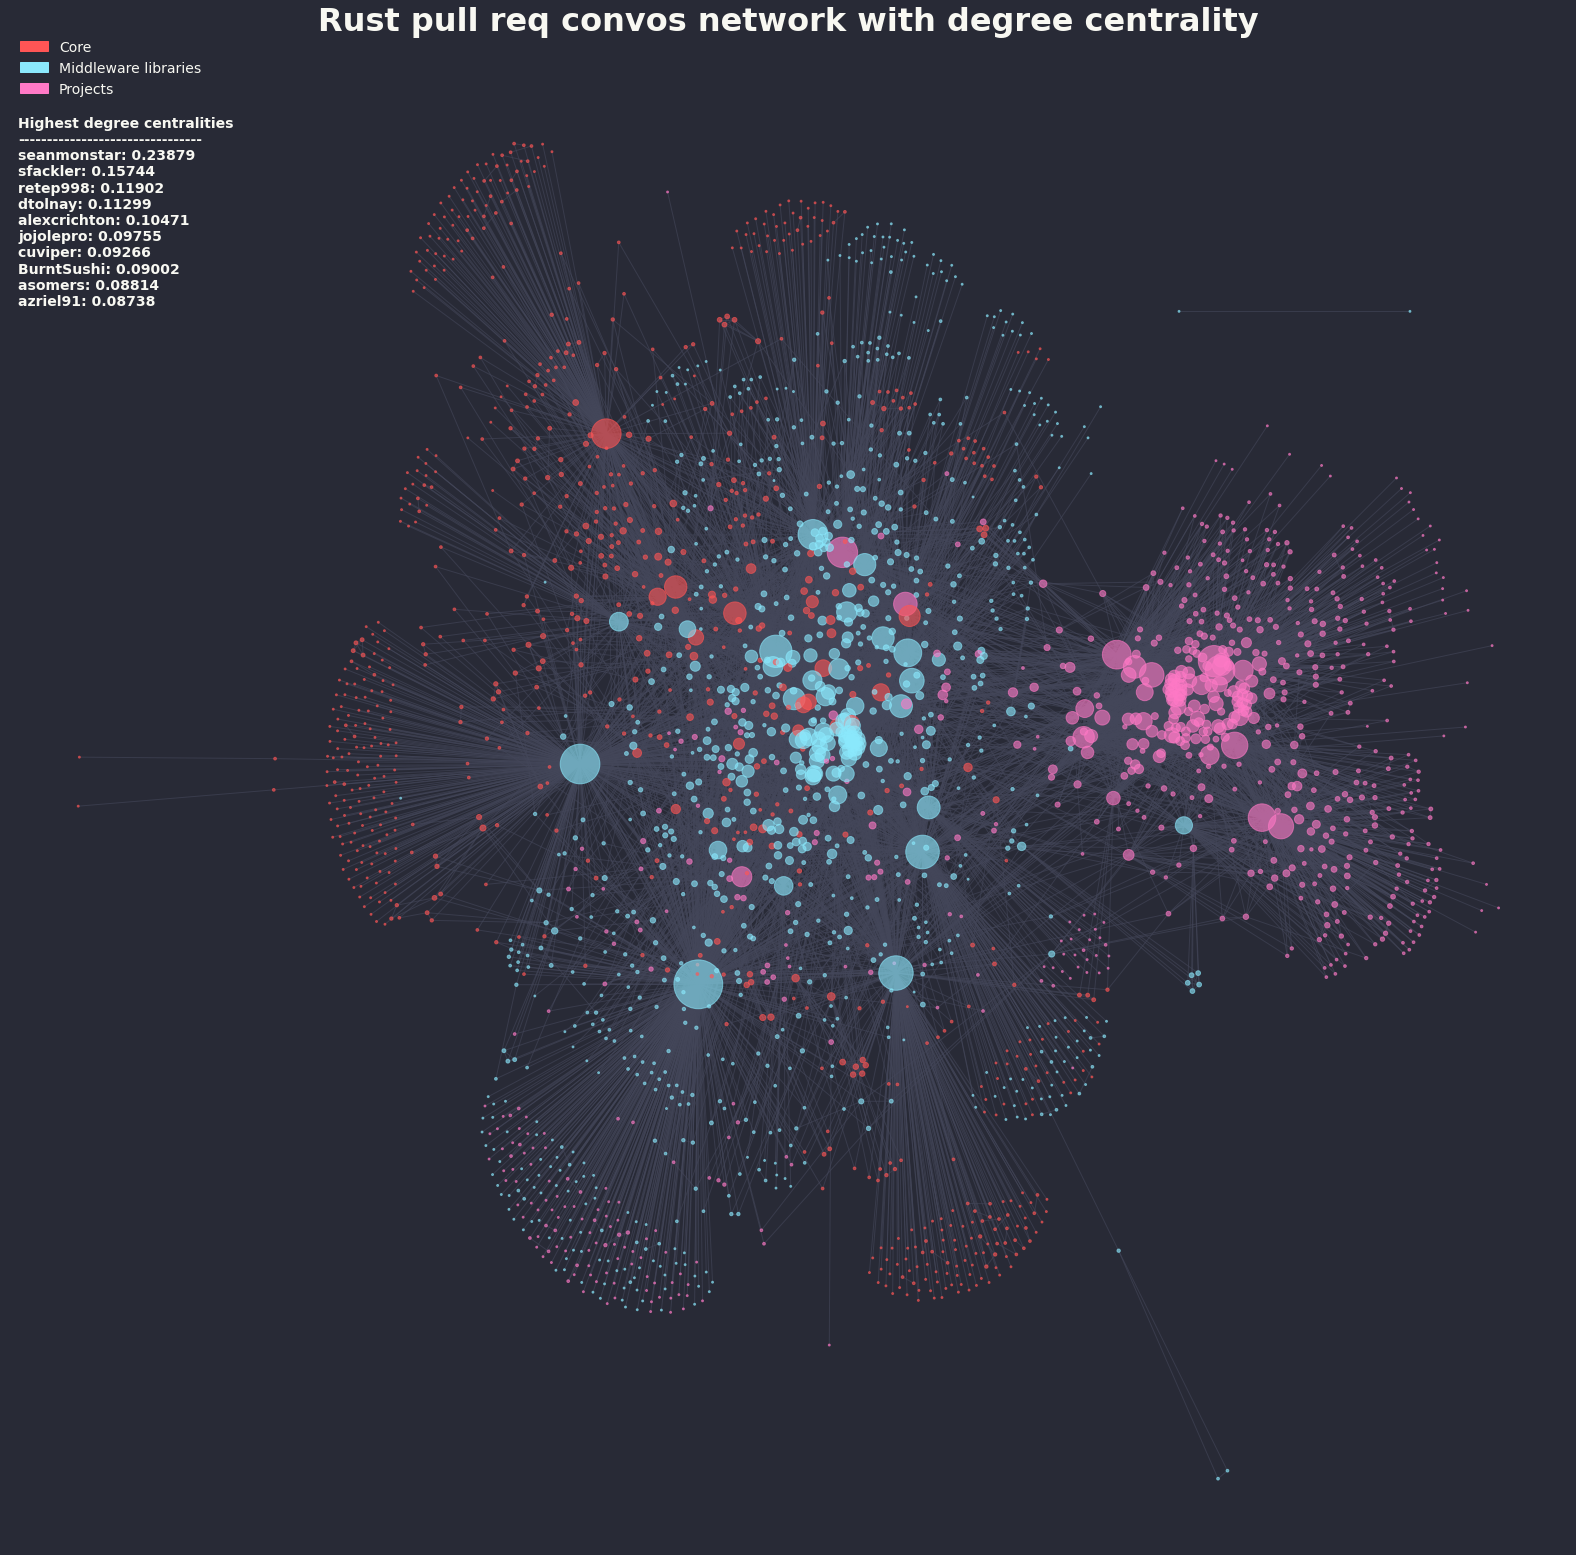
\includegraphics[width=\linewidth]{network_full_degcent.png}
    \caption{Full network projection of the PR network. Nodes are colored by attribute class, and size indicates degree centrality.}
    \label{fig:fullnet}
\end{figure}

\begin{table}
    \centering
    \begin{tabular}{ccc}
        \hline\\
        Metric & Full network & LCC\\
        \hline\\
        Nodes & 2656 & 2623\\
        Edges & 12302 & 12301\\
        Radius & $\infty$ & 3 (size: 9)\\
        Diameter & $\infty$ & 6 (size: 3)\\
        Clustering & 0.005134 & 0.005198\\
        Density & 0.003489 & 0.003577\\
        Degree assortativity & -0.250883 & -0.250925\\
        Most active assort & 0.461229 & 0.461189\\
        Max repo assort & 0.589387 & 0.589352\\
        Repo type assort & 0.576195 & 0.576170\\
        \hline
    \end{tabular}
    \caption{Metrics calculated via NetworkX for both the full network as well as the largest connected component. Radius and diameter are invalid for unconnected graphs. Repo type assort refers to the Core, Library, and Projects classes from earlier.}
    \label{tab:netresults}
\end{table}

Radius and diameter are interesting statistics that show node proximity. Radius and diameter measure closeness via eccentricity. Nodes with lower eccentricity are relatively closer to other nodes because they require less hops to reach them. I calculated radius using both NetworkX's default algorithm as well as using the barycenter metric. NetworkX's default algorithm finds nine nodes with the lowest eccentricity. Despite the myriad flaws explained earlier, most of the center nodes seem extremely reasonable. Names such as BurntSushi or David Tolnay are recognizable as pivotal Rustaceans. Reasonably, a Rust programmer who is aware of their contributions to the language would expect them to be closer to other nodes in some way by sheer inertia alone. These users tend to review PRs so they have a lot of spread in the community. Another user in the center, retep998, owns a major and useful repository: the Windows API bindings. That user also submitted PRs in some way to the random numbers, hyper, and OpenSSL bindings crates. The spread and centrality of these repositories means that retep998 is a clear center node. We could follow a similar logic for other users. Seanmonstar contributes to both hyper and reqwest which, again, provides a level of spread. The barycenter algorithm finds only David Tolnay as the most central node. Tolnay partook in PR conversations for several repository and is also a prominent Rustacean as mentioned earlier.

\begin{figure}[ht!]
    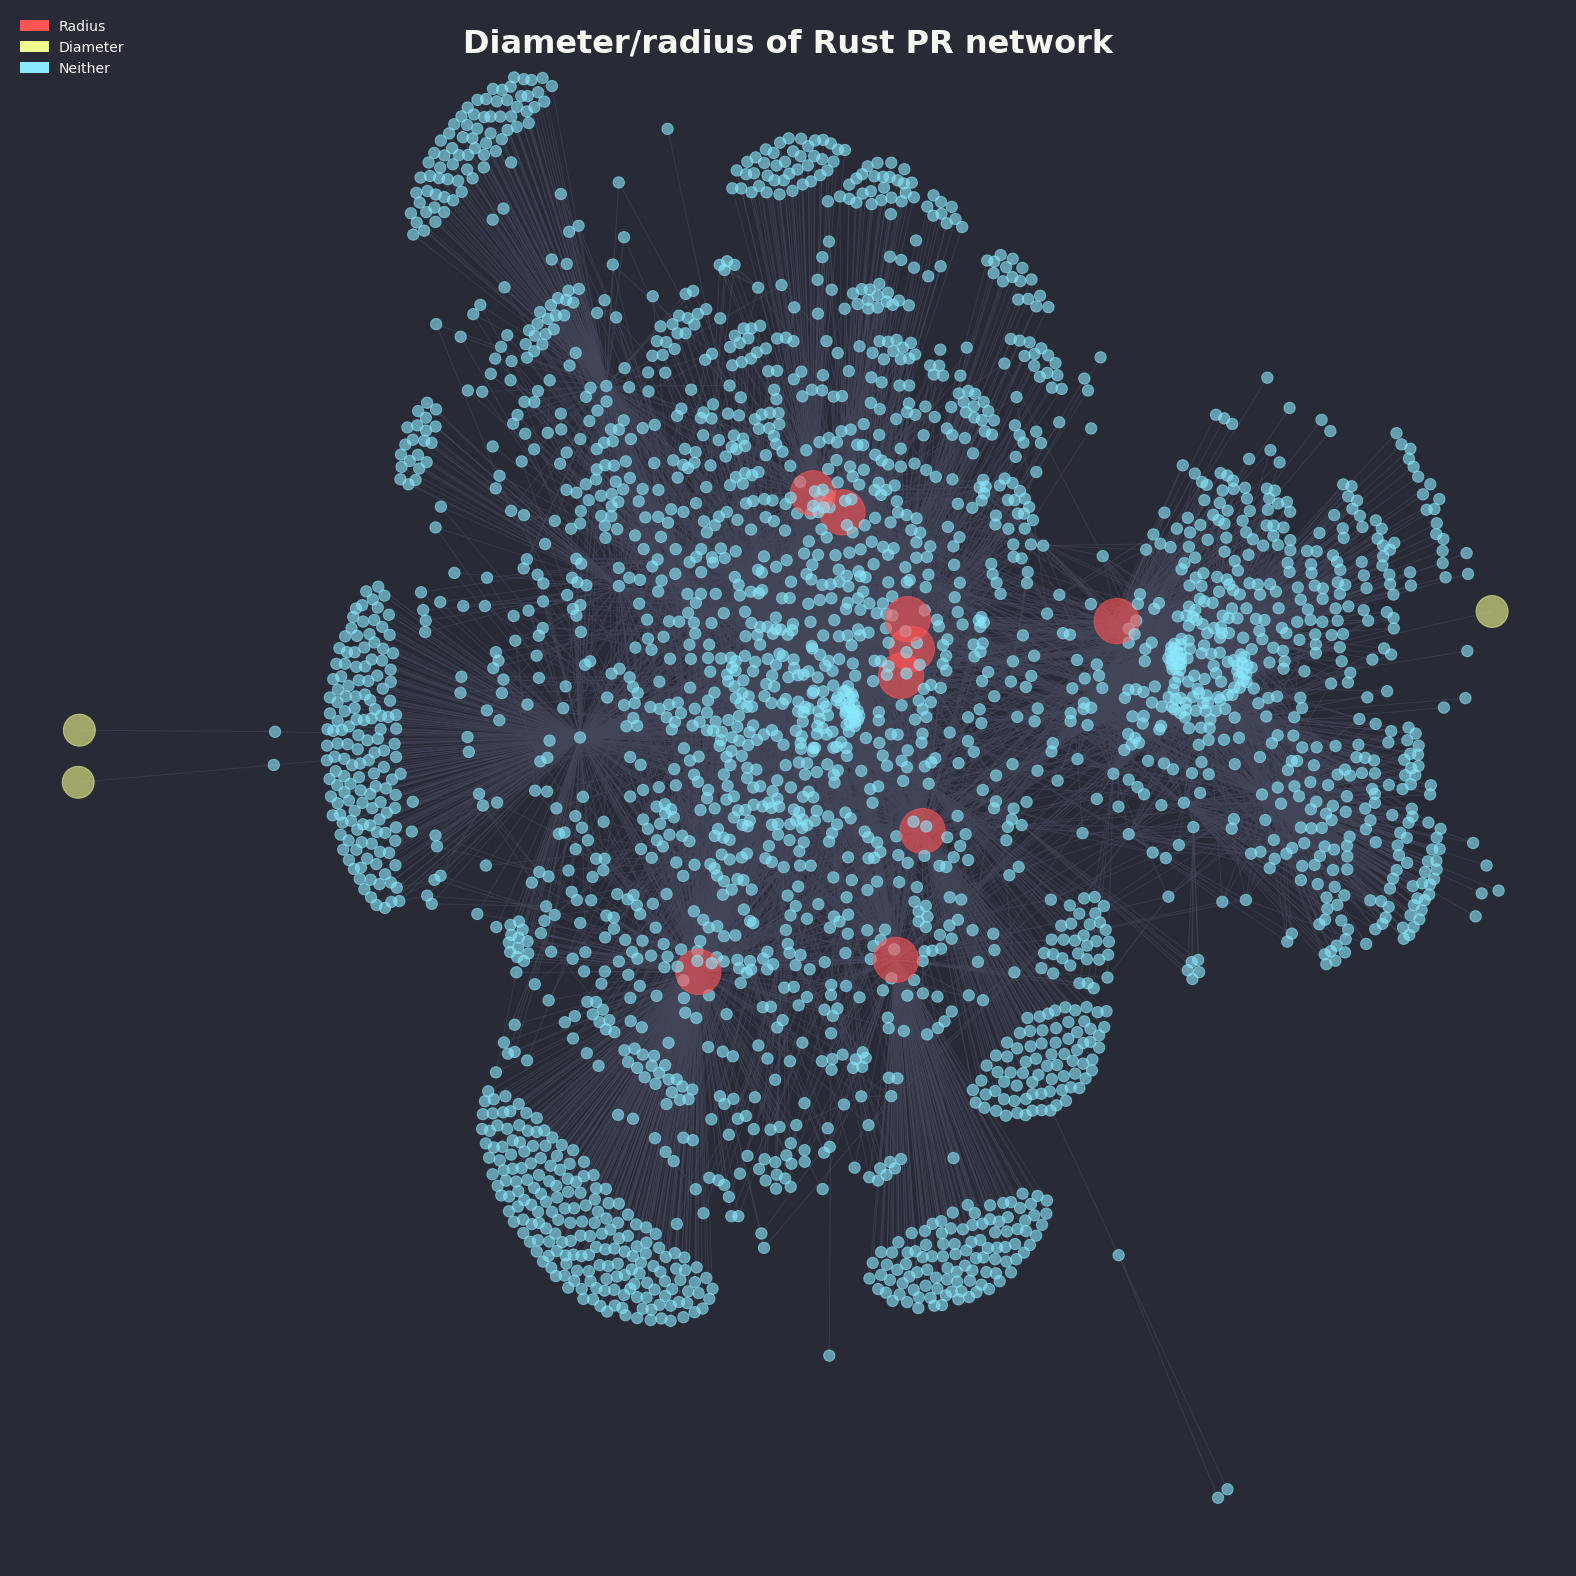
\includegraphics[width=\linewidth]{network_diarad.png}
    \caption{Diameter and radius of the Rust repository network.}
    \label{fig:diarad}
\end{figure}

The periphery or diameter contains only three nodes. These three nodes each have one PR conversation post in a PR that gathered little additional responses---usually from other highly eccentric individuals. A programmer who has little connections in a GitHub network (or any network) is likely to be deemed not pivotal.

\subsection{Clustering and density}
Clustering and density are expectedly both very low. Density, or the ratio of actual connections to total possible connections, measures how connected nodes are to all other nodes in the network. For social networks, including GitHub networks, we wouldn't expect high density because nodes are extremely unlikely to be connected to huge amounts of nodes. Clustering refers to triangles or triads where three nodes are connected. Average clustering is low as well and actually lower than expected when compared to a random graph. A PR conversation graph is heavily bridged by core members connecting other users who open pull requests. Therefore, PR graphs are likely to have lower transitivity than random or even compared to other social networks.

\subsection{Assortativity}
Degree assortativity measures the correlation of nodes with similar degrees sharing an edge. Interestingly, the correlation is moderately negative. The PR network is skewed by design in terms of degree. The count of users with very high degrees is much smaller than the count of external collaborators. In other words, we'd expect programmers with lower degrees (in terms of the Rust data) to be connected to users with high degrees (core members of a repository). Programmers with lower degrees are unlikely to respond often to other nodes with lower degrees in the network. Therefore, degree assortativity is negative.

Most active repository, max repository, and repo type assortativity all have moderately positive correlations. The interesting difference here is between most active versus max and repo type. Most active has a slightly lower correlation. Recall that most active selects the most active repository total for each user in terms of the data. Unfortunately, this distinction is possibly caused by our lack of data. The max repo per every user is one of the repositories scraped. However, if I gathered more data I would have all of the repositories where the node engaged in a PR conversation. The same flaw applies in a different way to my other assortativity measures. Assortativity would likely be vastly different with more classifications. However, for my coarse classifications, nodes tend to stay reasonably within their assigned class.

The plot of the full network shows both the tendency to engage with projects in the same class as well as the reasonable diversity of connections. Many of the nodes with high degree centrality are connected via a PR to nodes with different classes than their own. So, for example, some nodes contribute mainly to a library but have a lot of core connections---perhaps from their own PRs or from people who work on the core contributing to their library.

\begin{figure}[ht!]
    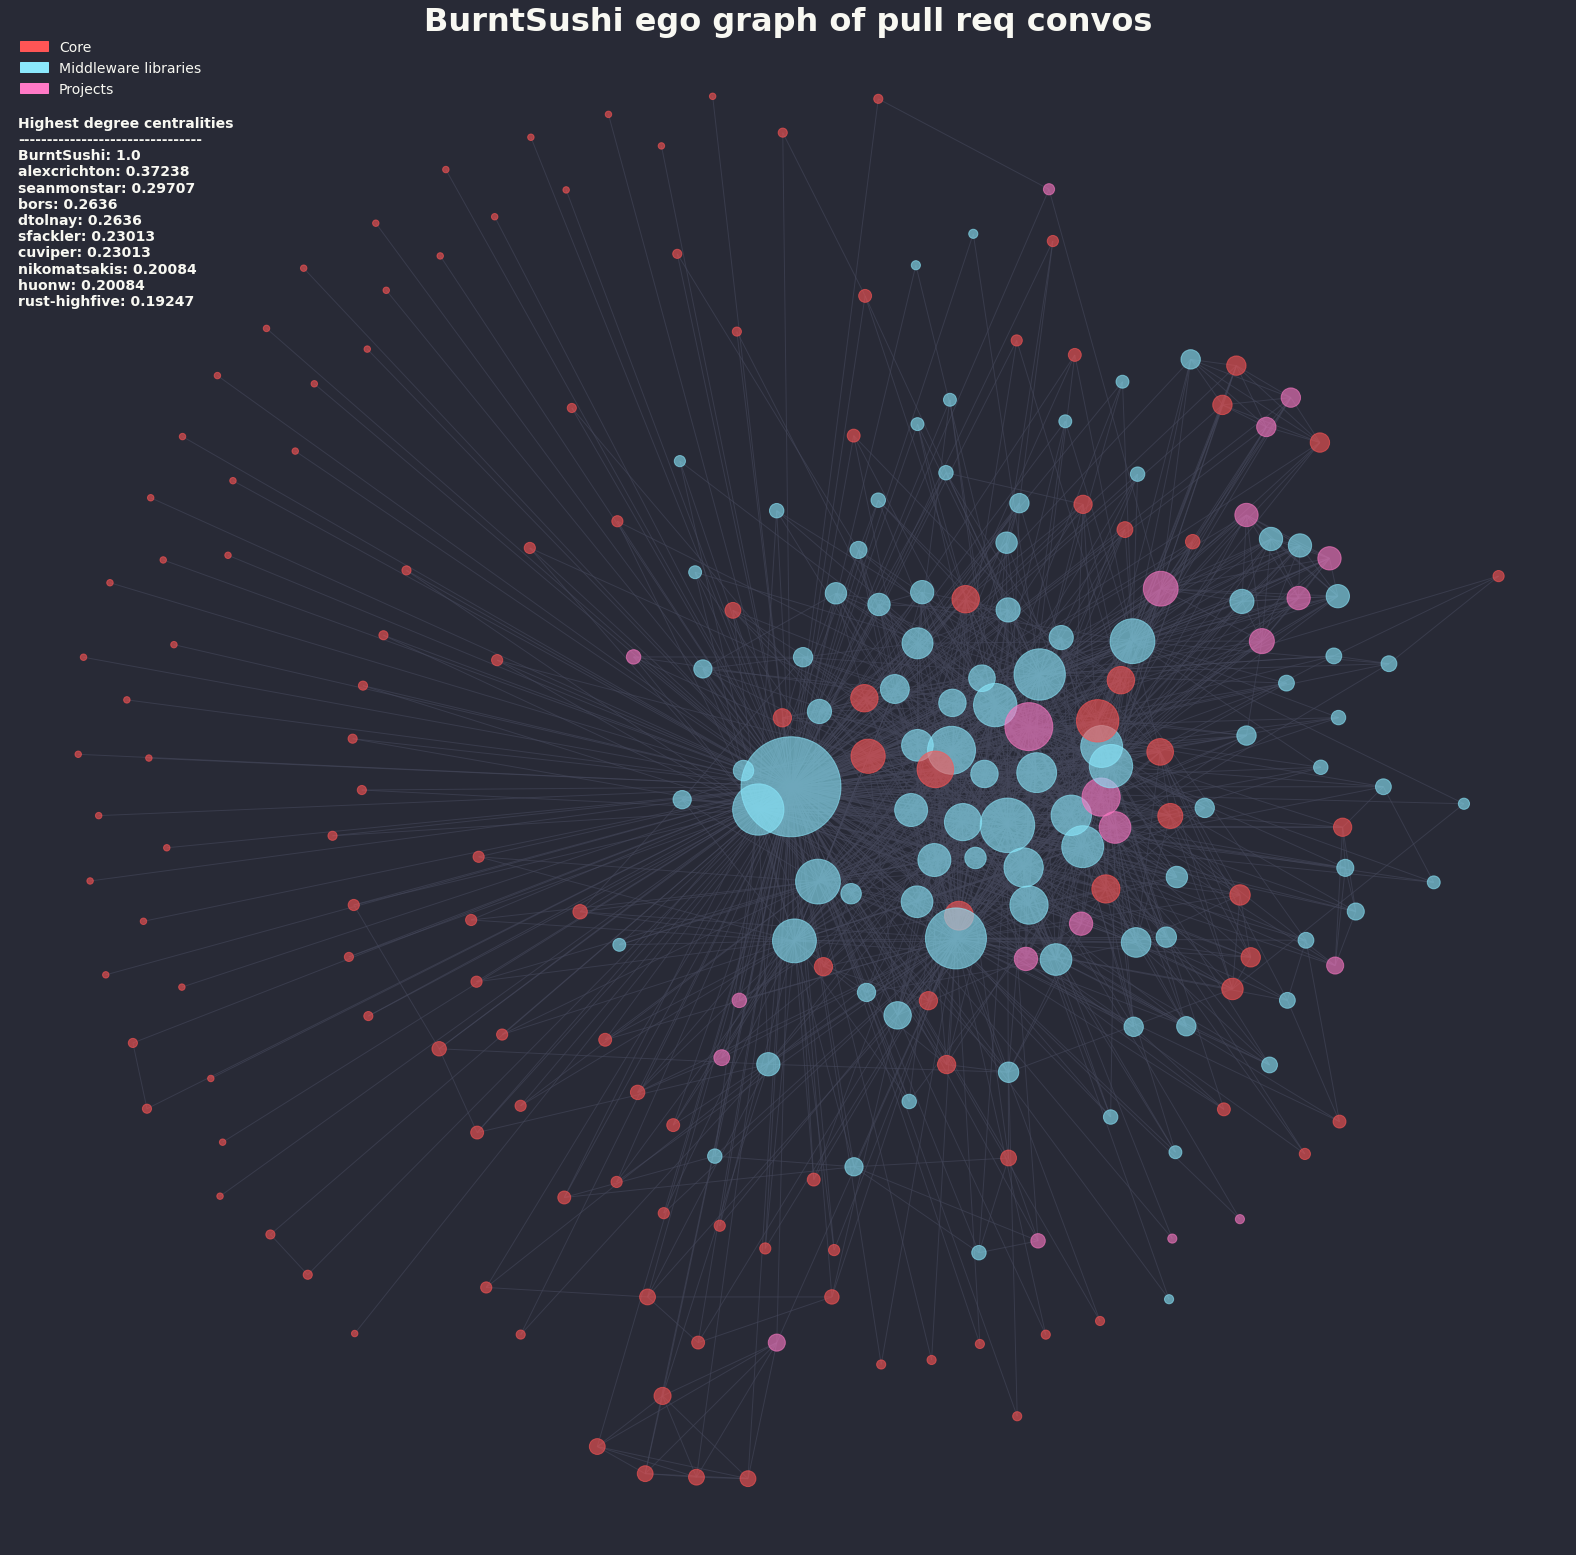
\includegraphics[width=\linewidth]{network_ego_degcent.png}
    \caption{BurntSushi's ego network. The diversity of connections is apparent when zoomed into one node.}
    \label{fig:burntego}
\end{figure}

An ego graph zooms into one node to show only their connections. The plot above zooms into BurntSushi. His ego graph shows a prevalent diversity of connections. Notably, this Rustacean does in fact work across all three coarse classes which provides both great spread (leading to closeness to other nodes) as well as multifaceted connections.

\section{Discussion}
My results were fairly interesting despite the fact that this is a flawed and small sample. I'd presume that many of the Rustaceans in the center would have a low eccentricity in the ideal full graph as well. For example, BurntSushi is prominent enough that most Rust programmers likely heard his username and real name as well as read at least one of his articles. His diverse contributions as well as the diversity in terms of programmers who likely submit PRs in a repository where he has privileges would mean that he would remain a pivotal node in the full network as well. Likewise, seanmonstar's reqwest and hyper are fairly standard crates for anyone who requires a simple, pragmatic HTTP client (reqwest) or something more powerful (hyper). I would presume programmers like seanmonstar are extremely pivotal based on my domain knowledge of Rust without even analyzing the network. Therefore, my network analysis confirms some of what I reasonably expected to be fact which in turn grants some credence to an obviously flawed study.

Some of the results, such as degree assortativity, are both logical and fascinating. A GitHub PR network is rather strange in terms of a social network. The network is heavily predicated on betweenness centrality\footnote{Not calculated because the algorithm is extremely slow with a lot of edges.} which is very visible in all of the graphs. High profile nodes act like gatekeepers in a sense. An important node that responds in the same PR as a less central node pulls that node very deep into the network by lowering their eccentricity. In other networks, like say Reddit or even Twitter, the amount of nodes with high degrees is more evenly spread out. "Super" nodes may exist that have a high in degree (say, celebrities) but nodes are not reliant on super nodes for embeddedness.

Future research\footnote{Much like my thesis} would require far more data as well as distributed computing or server class hardware to analyze. Perhaps the high performance algorithms can even be written in Rust!

\printbibliography
\end{document}
